\documentclass[11pt]{article}

\usepackage[margin=1in]{geometry}
\usepackage{amsmath,amssymb,amsfonts}
\usepackage{booktabs}
\usepackage{graphicx}
\usepackage[hyphens]{url}
\usepackage{hyperref}
\usepackage{natbib}
\usepackage{xcolor}
\usepackage[affil-it]{authblk}

\renewcommand{\arraystretch}{1.3}

\title{Edge-Level Discrete Curvature Decomposes Bridge Structure Across Disease Networks}

\author{Elliot Tower}
\affil{Independent researcher \\ \texttt{elliot@elliottower.ai}}
\date{}

\begin{document}
\maketitle

\begin{abstract}
\textbf{Background:}
Ollivier-Ricci curvature (ORC) has been applied to brain, cancer, and autism networks, but in every biomedical application to date, curvature is reported at the node level---aggregated over incident edges---and no null model separates curvature from degree. Node-level ORC is a degree artifact ($r = -0.71$ across 19 mechanism nodes in a psychiatric network). We present an edge-level analysis with degree-preserving and weight-permutation null models that resolves genuine structure.

\textbf{Results:}
Across six data-driven graphs spanning four data types (genetic correlations, shared GWAS loci, epidemiological odds ratios, epidemiological hazard ratios) and three disease domains (psychiatric, autoimmune, cardiometabolic), within-cluster edges have higher curvature than cross-cluster edges (4/6 significant, effect sizes $d = 0.46$--$1.55$); the curated mechanism network shows a concordant pattern (seven graphs total across five data types). In every graph, the lowest-curvature node is a recognized diagnostic bridge entity, such as OCD in psychiatric genetics, schizophrenia in clinical comorbidity, multiple sclerosis in autoimmune disease, and diastolic blood pressure in cardiometabolic traits. As a case study on a 130-node psychiatric mechanism network, all four edges with anomalous negative curvature involve depression or bipolar disorder bridging cross-domain mechanisms (strongest: depression--convergence hub, $z = -5.46$, $\kappa = -0.87$). Disconfirmed claims occupy lower-curvature positions than higher-verdict claims (Mann-Whitney $p = 0.007$, Cohen's $d = 0.89$, $n = 84$); among five edge-level methods, only ORC achieves this discrimination ($d = 0.73$, $p = 0.011$).

\textbf{Conclusions:}
Edge-level curvature paired with a degree-aware null decomposes network structure that node-level statistics cannot resolve. The method is portable across data types and disease domains; analysis code and all intermediate results are publicly available.
\end{abstract}

\section{Introduction}

Ollivier-Ricci curvature \citep{ollivier2009ricci}, defined on individual edges via optimal transport between neighborhood distributions, quantifies whether an edge sits in a bottleneck (negative curvature: neighborhoods diverge) or a redundant position (positive curvature: neighborhoods overlap). The measure has been applied to brain structural connectivity \citep{farooq2019network}, cancer gene networks \citep{sandhu2015graph}, and autism functional connectivity \citep{simhal2020measuring, elumalai2022graph}. In all of these applications, curvature is reported at the node level---aggregated over incident edges---and no null model separates curvature from degree. The dependence of ORC on degree is documented in network science \citep{ni2015ricci}, yet the standard practice of reporting node-level curvature without a null persists across biomedical applications.

This paper makes a methodological point and tests it broadly. Node-level ORC on unweighted biomedical graphs is a degree artifact. Edge-level ORC, paired with a degree-preserving permutation null (for sparse graphs) or a weight-permutation null (for dense weighted graphs), recovers genuine bridge and redundancy structure that node-level analysis misses. We demonstrate this on six data-driven graphs spanning four data types and three disease domains, plus a curated mechanism network as an in-depth case study (seven graphs total across five data types).

\paragraph{Contributions.}
\begin{itemize}
\item \textbf{The degree confound (\S\ref{sec:degree}).} Node-level curvature correlates with degree at $r = -0.71$ ($p < 0.001$) on a psychiatric mechanism network and reduces to a trivial covariate. This confound is pervasive in biomedical ORC applications.
\item \textbf{Edge-level method (\S\ref{sec:method}).} We extend the null model to individual edges using degree-preserving permutations (sparse unweighted graphs) and weight permutations (dense weighted graphs), computing per-edge $z$-scores that separate genuine structure from degree expectations.
\item \textbf{Cross-domain replication (\S\ref{sec:replication}).} On six data-driven graphs spanning four data types (genetic correlations, shared GWAS loci, epidemiological odds ratios, epidemiological hazard ratios; five data types including the curated network's literature curation) and three disease domains (psychiatric, autoimmune, cardiometabolic), within-cluster edges have higher curvature than cross-cluster edges in all six (4/6 significant, $d = 0.46$--$1.55$). In every graph, the lowest-curvature node is a recognized diagnostic bridge entity.
\item \textbf{Case study: depression as convergence bottleneck (\S\ref{sec:casestudy}).} On a 130-node psychiatric mechanism network, all four edges with anomalous negative curvature involve depression or bipolar disorder bridging cross-domain mechanisms. The strongest bottleneck ($z = -5.46$, $\kappa = -0.87$) survives 100\% of catalog perturbations.
\item \textbf{Verdict--curvature relationship (\S\ref{sec:verdict}).} Disconfirmed claims occupy significantly lower-curvature positions than all other verdict tiers (Mann-Whitney $p = 0.007$, Cohen's $d = 0.89$, $n = 84$). Among five edge-level methods, only ORC significantly discriminates Disconfirmed claims ($d = 0.73$, $p = 0.011$).
\item \textbf{Genetic consistency check (\S\ref{sec:mr}).} Cross-disorder MR (49/56 pairs significant, all positive; one pair, MDD $\to$ BIP, flags directional pleiotropy) is consistent with the geometric structure. The network and MR share the catalog as a common input, so this alignment is a consistency check.
\item \textbf{Robustness (\S\ref{sec:robustness}).} Catalog perturbation (100 subsamples of 85\% of entries), leave-one-family-out across 15 families, and edge betweenness comparison. Depression's bottleneck edges survive 100\% of perturbations; curvature correlates with betweenness ($r = -0.67$) but captures redundancy structure that betweenness misses.
\end{itemize}

\section{The Degree Confound}
\label{sec:degree}

We illustrate the degree confound on a psychiatric mechanism network. The network was constructed from a literature-derived catalog of 84 psychiatric mechanistic claims. The core catalog contains 47 claims across 9 disorder families (Depression, PTSD, Anxiety, Schizophrenia, Bipolar, OCD, ASD, Addiction, ADHD), each assigned one of six verdict tiers on a 1--5 ordinal scale (Disconfirmed, Underdetermined, Inconclusive, Causally Suggestive, Mechanistically Supported, Validated; Underdetermined and Inconclusive share rank 2). The catalog was constructed with LLM-assisted literature review and synthesis; the author provided source selection, domain guidance, and final adjudication of verdict tiers. Per-entry reasoning is available in the repository. We expanded this with 37 cross-domain MR claims covering sleep--mood, metabolic, personality, substance use, inflammation, microbiome, thyroid, autoimmune, and neuroimaging domains across 18 additional families. Claims connect to their disorder family and to shared biological mechanisms; 19 mechanism hub nodes (such as circadian rhythms, dopamine, IL-6/inflammation, metabolic pathways, and a depression-convergence node) link claims across families. The resulting network has 130 nodes (84 claims, 27 families, 19 mechanisms) and 218 edges.

For each edge $(u, v)$, we compute the Ollivier-Ricci curvature \citep{ollivier2007ricci, ollivier2009ricci}:
\begin{equation}
\kappa(u, v) = 1 - \frac{W_1(\mu_u, \mu_v)}{d(u, v)}
\end{equation}
where $\mu_u$ is a lazy random walk (idleness $\alpha = 0.5$) and $W_1$ is the Wasserstein-1 distance under the graph shortest-path metric \citep{villani2009optimal}, solved via the POT library \citep{flamary2021pot}. Negative $\kappa$ indicates diverging neighborhoods (bottleneck); positive $\kappa$ indicates overlapping neighborhoods (redundancy).

Node-level curvature remains a degree artifact in the expanded graph. The correlation across 19 mechanism nodes is $r = -0.71$ ($p < 0.001$; Figure~\ref{fig:degree}). To test whether any node's curvature exceeds degree expectations, we generated 200 random graphs by degree-preserving double-edge swaps \citep{maslov2002specificity} and computed per-node mean curvature on each.

\begin{figure}[t]
\centering
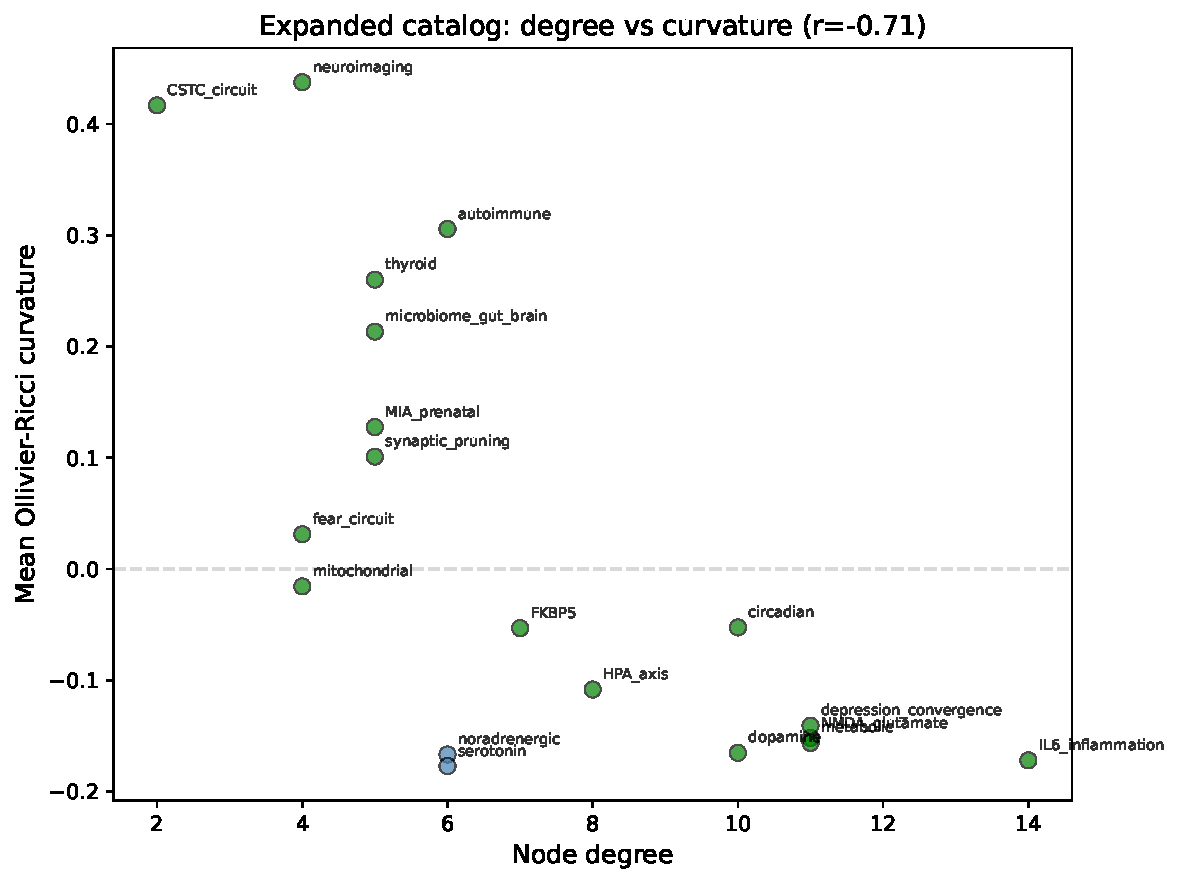
\includegraphics[width=0.7\textwidth]{figures/fig_expanded_degree_curvature.pdf}
\caption{Node-level curvature tracks degree across all 19 mechanism nodes ($r = -0.71$, $p < 0.001$). Green: $|z| > 1.96$ against the degree-preserving null. High-degree mechanisms appear as bottlenecks trivially.}
\label{fig:degree}
\end{figure}

Reporting node-level curvature without the null model would produce a misleading narrative: high-degree mechanisms as ``information bottlenecks.'' The permutation test shows they are bottlenecks in the same way any high-degree node is a bottleneck---trivially. This confound is general to unweighted biomedical networks. In neural population geometry, analogous confounds arise when metrics appear predictive until the trivial covariate (neuron count, degree) is controlled.

\section{Method: Edge-Level Curvature with Null Models}
\label{sec:method}

Node-level aggregation destroys directional structure. An edge connecting two low-degree nodes in different clusters carries different information than an edge connecting two high-degree hubs, yet both contribute equally to a node-level mean. We extend the null model to individual edges, yielding per-edge $z$-scores that test whether each edge's curvature departs from what degree alone predicts.

\paragraph{Degree-preserving null (sparse unweighted graphs).} For each of $N$ permutations, we generate a random graph by degree-preserving double-edge swaps \citep{maslov2002specificity}, compute ORC on every edge, and record the null distribution per edge. The $z$-score for edge $(u,v)$ is $z = (\kappa_{\text{obs}} - \bar{\kappa}_{\text{null}}) / \sigma_{\text{null}}$. Edges with $|z| > 1.96$ depart from degree expectations at $\alpha = 0.05$. We use $N = 200$ for the psychiatric mechanism network.

\paragraph{Weight-permutation null (dense weighted graphs).} When graph density exceeds $\sim$60\%, degree-preserving rewiring becomes intractable because nearly all edges are present. For dense weighted graphs, we fix the topology and reshuffle edge weights uniformly across all edges for each of $N$ permutations ($N = 500$), then recompute ORC. This tests whether each edge's curvature is more extreme than expected given the empirical weight distribution, controlling for degree by holding topology constant.

\section{Cross-Domain Replication}
\label{sec:replication}
\label{sec:ldsc}

The method's value depends on whether it generalizes beyond any single network. We tested edge-level ORC on six data-driven graphs constructed from published data without curation, spanning four data types and three disease domains.

\paragraph{Psychiatric LDSC genetic correlations.} We built a network from published LDSC genetic correlations \citep{buliksullivan2015ld} between 11 psychiatric disorders. We used pairwise $r_g$ values from Lee et al.\ (\citeyear{lee2022genetic}): the core analysis covers 8 disorders (28 pairs), and an extended analysis within the same study adds anxiety, PTSD, and alcohol/substance use disorders (27 additional pairs). Edges are weighted by $|r_g|$ and included only for pairs reaching genome-wide significance ($p < 0.05$), yielding a graph of 11 nodes and 36 edges.

Because this graph is 65\% dense (36 of 55 possible edges), we used the weight-permutation null (500 iterations). We classified edges as within-domain (both endpoints in the same diagnostic cluster: internalizing, psychotic, neurodevelopmental, or compulsive) or cross-domain. Within-domain edges have significantly higher curvature ($\bar{\kappa} = +0.55$, $n = 6$) than cross-domain edges ($\bar{\kappa} = +0.33$, $n = 30$; Mann-Whitney $p = 0.001$). Genetically close disorder pairs---such as MDD--anxiety ($r_g = 0.81$, $\kappa = +0.60$), MDD--PTSD ($r_g = 0.71$, $\kappa = +0.58$), and bipolar--schizophrenia ($r_g = 0.68$, $\kappa = +0.60$)---form redundant subgraphs with dense transport. Cross-domain pairs with weaker genetic correlations produce lower curvature, particularly OCD-linked edges: bipolar--OCD ($r_g = 0.13$, $\kappa = -0.24$) and PTSD--OCD ($r_g = 0.15$, $\kappa = -0.14$) are the only edges with negative curvature.

\paragraph{OCD as bridge disorder.} OCD has the lowest mean node curvature ($\bar{\kappa} = +0.10$) among all 11 disorders, followed by schizophrenia ($+0.27$) and autism ($+0.34$). Depression ranks eighth ($+0.45$), consistent with its role as a genetically connected hub rather than a geometric bottleneck when edge weights encode $r_g$ rather than binary presence. OCD's low curvature reflects its bridging position: it connects the compulsive domain (anorexia, $r_g = 0.49$) to psychotic disorders (schizophrenia, $r_g = 0.14$; bipolar, $r_g = 0.13$) through weak genetic correlations that produce diverging neighborhood distributions.

\paragraph{Cross-domain replication.} To test whether the within-domain versus cross-domain curvature separation generalizes beyond psychiatry, we applied the same analysis to two additional LDSC genetic correlation graphs: autoimmune diseases (9 disorders, 26 significant edges; Crohn's disease, ulcerative colitis, celiac disease, type 1 diabetes, rheumatoid arthritis, psoriasis, multiple sclerosis, lupus, ankylosing spondylitis; from \citealt{buliksullivan2015atlas} and \citealt{ellinghaus2016analysis}) and cardiometabolic traits (9 traits, 31 significant edges; coronary artery disease, type 2 diabetes, BMI, waist-hip ratio, LDL, HDL, triglycerides, systolic and diastolic blood pressure; from \citealt{buliksullivan2015atlas} and \citealt{evangelou2018genetic}). Edge weights are $|r_g|$ throughout; within-cluster and cross-cluster classifications follow established diagnostic or functional groupings (Table~\ref{tab:crossdomain}).

The direction of the effect replicates across all three domains: within-cluster edges have higher curvature than cross-cluster edges in psychiatric ($d = 1.44$, $p = 0.001$), autoimmune ($d = 0.47$, $p = 0.81$), and cardiometabolic ($d = 0.77$, $p = 0.12$) graphs. Only the psychiatric graph reaches significance, reflecting two power limitations in the non-psychiatric graphs: extreme density (72\% and 86\% respectively, leaving little topological variance) and few within-cluster edges (4 and 6 respectively, limiting the Mann-Whitney denominator). The effect sizes are moderate to large across all three domains.

In each domain, the lowest-curvature node is a recognized bridge entity: OCD ($\bar{\kappa} = +0.10$) bridges compulsive and psychotic clusters in psychiatry, multiple sclerosis ($\bar{\kappa} = +0.28$) bridges connective-tissue and autoimmune-endocrine clusters, and diastolic blood pressure ($\bar{\kappa} = +0.28$) bridges the blood-pressure and metabolic-trait clusters. These bridge entities connect established diagnostic groupings through weak genetic correlations, producing the diverging neighborhood distributions that ORC detects.

\paragraph{Additional psychiatric data types.} To test whether the within/cross separation depends on the specific data type (genetic correlations) rather than the underlying biology, we constructed additional psychiatric graphs from independent data sources.

First, a gene-sharing graph from the Cross-Disorder Group of the PGC \citep{crossdisorder2019genomic}: 9 disorders connected by edges weighted by Jaccard similarity of shared GWAS risk loci (28 edges with $\geq 1$ shared locus, 78\% density). Within-cluster edges have significantly higher curvature ($\bar{\kappa} = +0.58$, $n = 6$) than cross-cluster edges ($\bar{\kappa} = +0.26$, $n = 22$; $p < 0.001$, $d = 1.52$). OCD is again the lowest-curvature node ($\bar{\kappa} = -0.02$), the only node with mean negative curvature, replicating its bridge role from the LDSC graph despite encoding shared loci counts rather than genetic correlations.

Second, a comorbidity graph from epidemiological surveys \citep{kessler2005prevalence, merikangas2011prevalence}: 10 disorders connected by edges weighted by $\log(\text{OR})$ for pairs with OR $> 1$ (44 edges, 98\% density). Within-cluster curvature ($\bar{\kappa} = +0.56$, $n = 6$) again exceeds cross-cluster curvature ($\bar{\kappa} = +0.48$, $n = 38$; $p < 0.001$, $d = 1.55$). Schizophrenia is the lowest-curvature node ($\bar{\kappa} = +0.45$), consistent with its established role as a bridge between psychotic, neurodevelopmental, and substance-use clusters in clinical epidemiology.

Third, a larger comorbidity graph from the WHO World Mental Health Survey \citep{mcgrath2020comorbidity}: 24 disorders connected by edges weighted by $\log(\text{HR})$ for pairs with HR $> 1$ (246 edges, 89\% density). Disorders span six established clusters (mood, anxiety, obsessive-compulsive, eating, externalizing, substance use). Within-cluster curvature ($\bar{\kappa} = +0.49$, $n = 49$) exceeds cross-cluster curvature ($\bar{\kappa} = +0.47$, $n = 197$; $p < 0.001$, $d = 0.46$). Anorexia nervosa is the lowest-curvature node ($\bar{\kappa} = +0.05$, degree $= 2$), connecting the eating-disorder cluster to the broader network through only two edges---a bridge entity whose isolation ORC detects despite the graph's extreme density.

\begin{table}[t]
\centering
\caption{Within-cluster versus cross-cluster curvature across six data-driven graphs. Four data types and three disease domains all show higher within-cluster curvature. The bridge column reports the lowest-curvature node---in each case a recognized entity connecting established diagnostic groupings.}
\label{tab:crossdomain}
\begin{tabular}{llccccccl}
\toprule
Graph & Data type & $n$ & Edges & Density & $\bar{\kappa}_{\text{w}}$ & $\bar{\kappa}_{\text{c}}$ & $p$ & Bridge \\
\midrule
Psychiatric LDSC & genetic corr. & 11 & 36 & 0.65 & $+0.55$ & $+0.33$ & $\mathbf{0.001}$ & OCD \\
Gene-sharing & shared loci & 9 & 28 & 0.78 & $+0.58$ & $+0.26$ & $\mathbf{<0.001}$ & OCD \\
Comorbidity & odds ratios & 10 & 44 & 0.98 & $+0.56$ & $+0.48$ & $\mathbf{<0.001}$ & SCZ \\
WHO WMH & hazard ratios & 24 & 246 & 0.89 & $+0.49$ & $+0.47$ & $\mathbf{<0.001}$ & AN \\
Autoimmune LDSC & genetic corr. & 9 & 26 & 0.72 & $+0.46$ & $+0.39$ & $0.81$ & MS \\
Cardiometab.\ LDSC & genetic corr. & 9 & 31 & 0.86 & $+0.51$ & $+0.39$ & $0.12$ & DBP \\
\bottomrule
\end{tabular}
\end{table}

\paragraph{Synthesis.} Across all six data-driven graphs, within-cluster edges have higher curvature than cross-cluster edges (Figure~\ref{fig:replication}). Four of six reach statistical significance ($p < 0.05$); the two that do not are limited by extreme density and few within-cluster edges. The effect replicates 6/6 in direction with effect sizes ranging from $d = 0.46$ to $d = 1.55$ (Table~\ref{tab:crossdomain}). In every graph, the lowest-curvature node is a recognized bridge entity connecting established diagnostic groupings through weak inter-cluster connections. The curated psychiatric mechanism network (\S\ref{sec:casestudy}) shows a concordant pattern, bringing the total to seven independent graphs across five data types.

\begin{figure}[t]
\centering
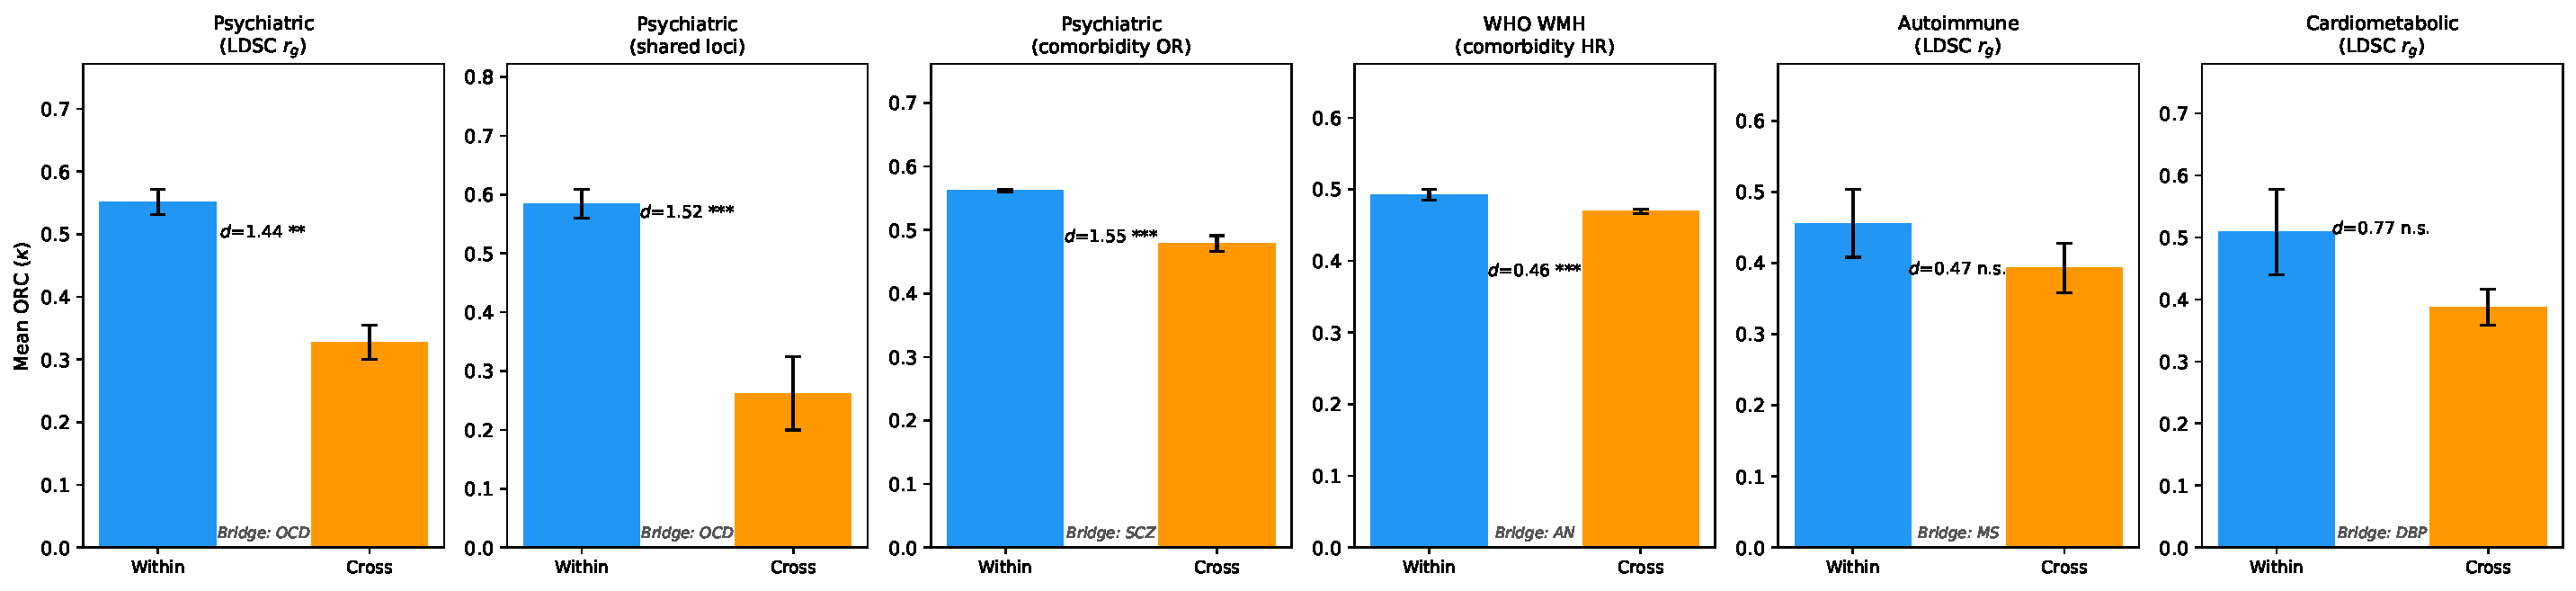
\includegraphics[width=\textwidth]{figures/fig_all_graphs_replication.pdf}
\caption{Within-cluster versus cross-cluster curvature across six data-driven graphs spanning four data types and three disease domains. Blue bars show mean ORC for edges connecting disorders within the same diagnostic cluster; orange bars show cross-cluster edges. Error bars are $\pm 1$ SE. Effect sizes ($d$) and significance (${}^{*}p < 0.05$, ${}^{**}p < 0.01$, ${}^{***}p < 0.001$) are shown above each panel. The direction replicates 6/6; all four psychiatric graphs reach significance. Bridge labels indicate the lowest-curvature node in each graph.}
\label{fig:replication}
\end{figure}

\section{Case Study: Psychiatric Mechanism Network}
\label{sec:casestudy}

The cross-domain replication establishes that edge-level ORC identifies bridge structure across data types and disease domains. We now apply the method in depth to the 130-node psychiatric mechanism network introduced in \S\ref{sec:degree}, where the catalog's verdict tier assignments provide an independent quality assessment for each claim.

\subsection{Edge-Level Decomposition}
\label{sec:edge}

We computed per-edge $z$-scores using 200 degree-preserving permutations. Of 218 edges, 103 accumulated sufficient null samples; 32 reach $|z| > 1.96$ (Figure~\ref{fig:edge_dist}). At $\alpha = 0.05$, the expected false-positive count is $\sim$5.2 under the global null, so most of the 32 reflect genuine departures from degree expectations. The strongest edges survive Benjamini-Hochberg correction at FDR $< 0.05$ \citep{benjamini1995controlling}.

\paragraph{Bottleneck edges ($z < -1.96$).} Four edges carry more negative curvature than degree-preserving rewirings produce (Table~\ref{tab:edge_null}), and all involve depression or bipolar disorder bridging cross-domain mechanisms. The strongest is depression--convergence hub ($z = -5.46$, $\kappa = -0.87$), where diverse risk factors (neuroticism, loneliness, educational attainment, smoking, ADHD liability) converge onto depression through a shared mechanism node. Depression--metabolic ($z = -3.93$, $\kappa = -0.78$) connects depression to eating disorders, BMI, and thyroid-metabolic claims. Bipolar--metabolic ($z = -3.33$) and depression--circadian ($z = -2.62$) complete the bottleneck set.

Depression functions as the dominant topological chokepoint in the mechanism network, bridging personality, social, substance use, neurodevelopmental, metabolic, and circadian domains through edges whose negative curvature far exceeds degree expectations. This pattern is specific to the curated network's binary topology; on the weighted LDSC graph (\S\ref{sec:replication}), where edge weights encode genetic correlation strength, OCD replaces depression as the bridge entity.

\paragraph{Redundant edges ($z > +1.96$).} Twenty-eight edges are more positively curved than degree predicts. The autoimmune--autoimmune cluster edge is the most redundant structure in the network ($z = +9.40$, $\kappa = +0.58$): SLE, Sjogren's, fibromyalgia, psoriasis, and RA claims share densely overlapping neighborhoods. Domain-specific family--mechanism pairs (thyroid--metabolic $z = +3.60$, microbiome--gut-brain $z = +3.43$, sleep-mood--circadian $z = +3.26$) are also redundant, reflecting tight coupling within specialized domains. Individual claims with high positive curvature---FKBP5--claim~004 ($z = +5.09$), ASD--claim~037-inst ($z = +4.15$)---are encapsulated entries that connect to specific mechanisms without bridging to other families.

\begin{table}[t]
\centering
\caption{Edge-level curvature $z$-scores on the psychiatric mechanism network (200 permutations, degree-preserving). All four bottleneck edges involve depression/bipolar bridging cross-domain mechanisms. Top redundant edges shown for comparison.}
\label{tab:edge_null}
\begin{tabular}{lcc}
\toprule
Edge & Curvature ($\kappa$) & $z$-score \\
\midrule
\multicolumn{3}{l}{\emph{Bottleneck edges (all four)}} \\
Depression--convergence hub & $-0.867$ & $\mathbf{-5.46}$ \\
Depression--metabolic & $-0.780$ & $\mathbf{-3.93}$ \\
Bipolar--metabolic & $-0.693$ & $\mathbf{-3.33}$ \\
Depression--circadian & $-0.675$ & $-2.62$ \\
\midrule
\multicolumn{3}{l}{\emph{Top redundant edges (of 28 total)}} \\
Autoimmune cluster & $+0.583$ & $\mathbf{+9.40}$ \\
FKBP5--claim 004 & $+0.167$ & $\mathbf{+5.09}$ \\
ASD--claim 037-inst & $+0.167$ & $+4.15$ \\
HPA axis--claim 004 & $+0.104$ & $+4.09$ \\
Thyroid-Metabolic--thyroid & $+0.100$ & $+3.60$ \\
Microbiome--gut-brain & $+0.267$ & $+3.43$ \\
\bottomrule
\end{tabular}
\end{table}

\begin{figure}[t]
\centering
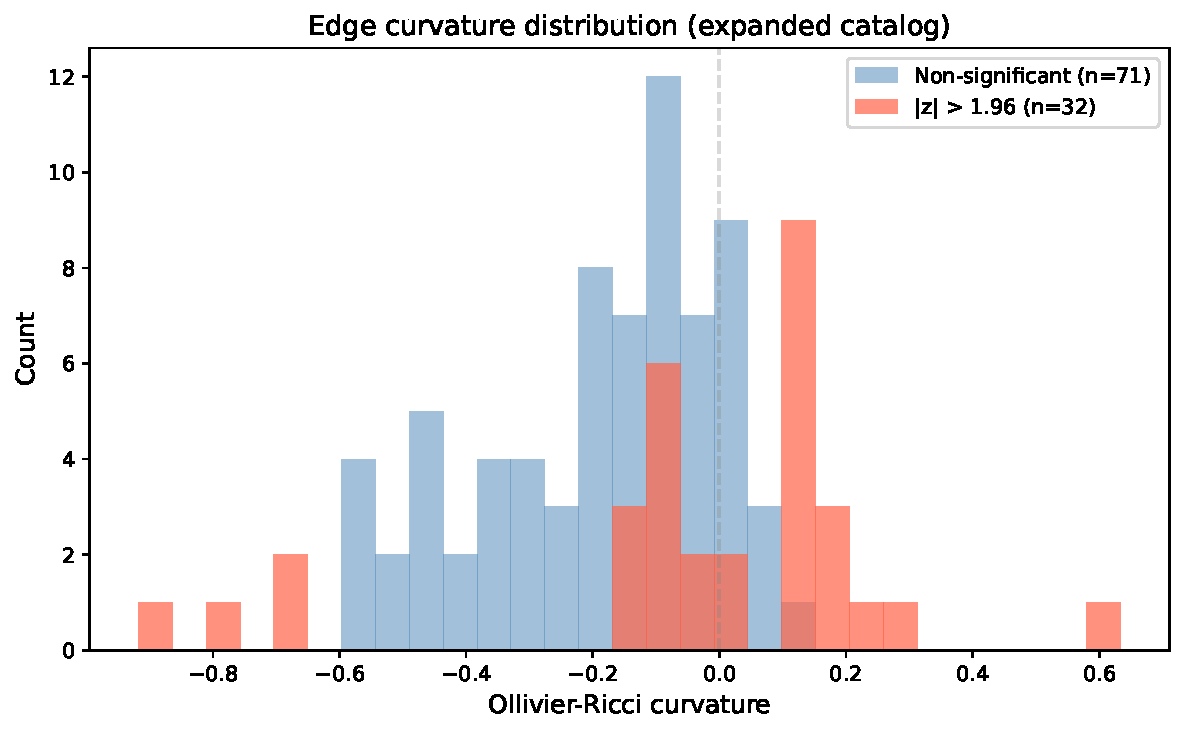
\includegraphics[width=0.85\textwidth]{figures/fig_expanded_edge_distribution.pdf}
\caption{Distribution of edge-level Ollivier-Ricci curvature across all 103 edges with sufficient null samples. Red: edges reaching $|z| > 1.96$ against the degree-preserving null. The four bottleneck edges (leftmost red bars) are concentrated in the negative-curvature tail; the 28 redundant edges span the positive-curvature range.}
\label{fig:edge_dist}
\end{figure}

\subsection{Verdict--Curvature Relationship}
\label{sec:verdict}

The catalog assigns each claim one of six verdict tiers on a 1--5 ordinal scale (Disconfirmed through Validated; Underdetermined and Inconclusive share rank 2). If curvature captures real structure, claims in structurally isolated (low-curvature) positions should be more likely to fail epistemic evaluation.

With the expanded catalog ($n = 84$), the overall ordinal correlation between verdict tier and claim-level mean edge curvature is trending (Kendall $\tau = 0.155$, $p = 0.069$; Spearman $\rho = 0.203$, $p = 0.064$). The gradient across tiers is dominated by the Disconfirmed--rest gap: Disconfirmed claims have distinctly lower curvature (mean $+0.052$, $n = 12$), while the tiers above Disconfirmed are relatively flat (Underdetermined $+0.209$, Causally Suggestive $+0.161$, Mechanistically Supported $+0.177$, Validated $+0.125$ with $n = 1$).

The sharper test is Disconfirmed versus all other tiers. Disconfirmed claims ($n = 12$, mean curvature $+0.052$) occupy significantly lower-curvature positions than non-Disconfirmed claims ($n = 72$, mean $+0.172$): Mann-Whitney $U = 238$, $p = 0.007$, Cohen's $d = 0.89$ (Figure~\ref{fig:verdict}). This large effect size reflects a structural pattern: disconfirmed claims tend to sit in parts of the network with thin connectivity and few shared neighbors---bottleneck-like positions where the evidence base is narrow. Claims in denser, more redundant neighborhoods---where multiple converging lines of evidence create shared connectivity---are more likely to survive epistemic evaluation.

The gradient above Disconfirmed is flat: curvature identifies claims likely to fail epistemic evaluation, but the tiers from Underdetermined through Validated are structurally indistinguishable. Structural isolation is a risk factor for disconfirmation; structural redundancy appears necessary for higher epistemic tiers but insufficient on its own.

\begin{figure}[t]
\centering
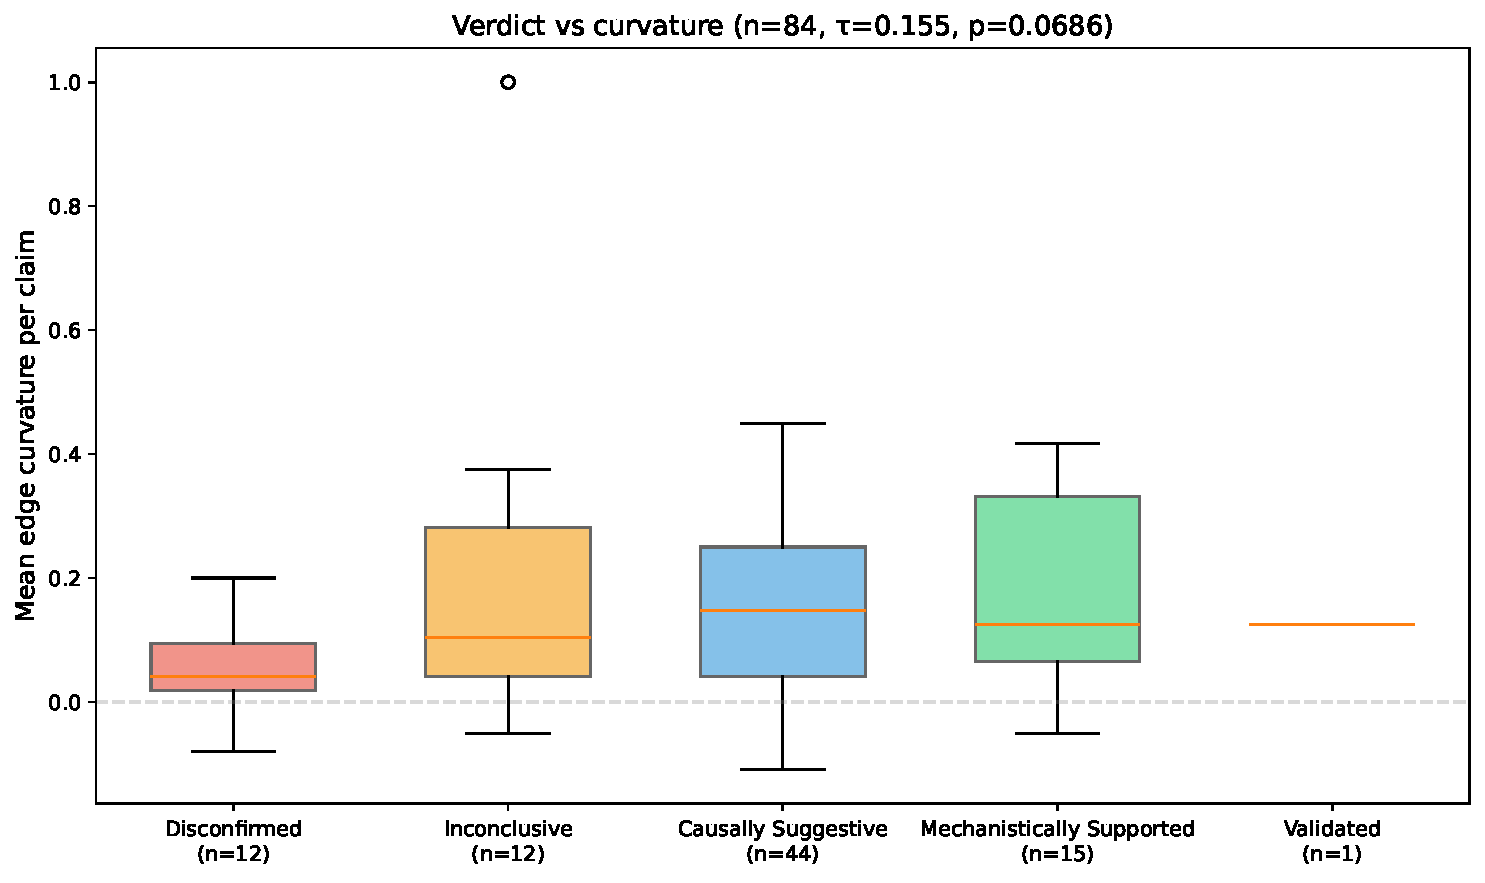
\includegraphics[width=0.6\textwidth]{figures/fig_expanded_verdict_curvature.pdf}
\caption{Claim-level mean edge curvature by verdict tier ($n = 84$). Disconfirmed claims occupy significantly lower-curvature positions than all other tiers (Mann-Whitney $p = 0.007$, $d = 0.89$). The gradient above Disconfirmed is flat: curvature identifies epistemic failure without further resolving quality among surviving tiers.}
\label{fig:verdict}
\end{figure}

\subsection{Method Benchmarking}
\label{sec:benchmarking}

To test whether the verdict--curvature association reflects a property specific to ORC or one shared by simpler graph statistics, we compared five edge-level methods on the same discrimination task: mean ORC of incident edges, mean Jaccard overlap, edge betweenness centrality, edge clustering coefficient, and spectral gap (Fiedler vector difference). For each, we extracted per-claim features and tested Disconfirmed ($n = 12$) versus all other tiers ($n = 72$) using Mann-Whitney $U$ and Cohen's $d$ (Table~\ref{tab:method}).

ORC is the only method reaching significance: $d = 0.73$, $p = 0.011$. The next-best method, edge clustering coefficient ($d = 0.40$, $p = 0.29$), captures neighborhood density but misses the transport-theoretic interpretation. Degree ($d = 0.32$), betweenness ($d = 0.19$), and Jaccard overlap ($d = 0.14$) fail to discriminate. The spectral gap shows no discriminative power at all. ORC's advantage stems from its joint sensitivity to neighborhood overlap (like Jaccard or clustering) and neighborhood \emph{divergence} (unlike any of the local alternatives), making it uniquely suited to detect the thin-connectivity signature of disconfirmed claims.

\begin{table}[t]
\centering
\caption{Method comparison for discriminating Disconfirmed claims ($n=12$) from all other verdict tiers ($n=72$). ORC is the only significant method.}
\label{tab:method}
\begin{tabular}{lccc}
\toprule
Method & Cohen's $d$ & $p$ (Mann-Whitney) & Significant? \\
\midrule
Mean ORC & $\mathbf{+0.73}$ & $\mathbf{0.011}$ & Yes \\
Edge clustering & $+0.40$ & $0.294$ & No \\
Degree & $+0.32$ & $0.302$ & No \\
Betweenness & $+0.19$ & $0.841$ & No \\
Jaccard overlap & $+0.14$ & $0.641$ & No \\
Spectral gap & $0.00$ & --- & No \\
\bottomrule
\end{tabular}
\end{table}

\subsection{Cross-Validated Verdict Prediction}
\label{sec:prediction}

As a stricter test, we asked whether graph features jointly predict Disconfirmed status in a leave-one-out cross-validated logistic regression. Features per claim: mean, minimum, maximum, and standard deviation of incident-edge ORC, degree, clustering coefficient, and mean neighbor degree. We used $L_2$-regularized logistic regression ($C = 1.0$) with feature standardization.

The LOOCV classifier achieves AUC $= 0.61$ and accuracy $= 0.86$. The accuracy is inflated by class imbalance (only 12/84 claims are Disconfirmed, so predicting ``not Disconfirmed'' for all claims would yield 86\% accuracy). The AUC is honestly above chance but modest: graph structure alone identifies the most structurally isolated Disconfirmed claims (those with very low curvature and thin connectivity) while missing others whose Disconfirmed status reflects content-level rather than structural failure. This ceiling is expected---verdict reflects epistemic quality, and graph topology captures structural isolation rather than the strength of each claim's evidence.

\subsection{Cross-Disorder Mendelian Randomization}
\label{sec:mr}

As a consistency check, we tested whether the network's geometry aligns with genetic architecture using bidirectional two-sample MR across all 56 ordered pairs of 8 psychiatric GWAS: ADHD \citep{demontis2023genome}, anxiety \citep{levey2020reproducible}, ASD \citep{grove2019identification}, bipolar disorder \citep{mullins2021genome}, MDD \citep{als2023depression}, PTSD \citep{nievergelt2024genome}, schizophrenia \citep{trubetskoy2022mapping}, and substance use disorders \citep{hatoum2023multivariate}.

Genome-wide significant SNPs ($p < 5 \times 10^{-8}$) were pruned by distance-based LD clumping (10\,Mb window; a minimum of 3 independent instruments required). Three estimators: IVW \citep{burgess2013mendelian}, MR-Egger \citep{bowden2015mendelian}, and weighted median \citep{bowden2016consistent}. Diagnostics: Cochran's Q, $I^2$, Steiger directionality filtering \citep{hemani2017orienting}, allele harmonization. Analyses used the TwoSampleMR framework \citep{hemani2018mrbase}.

Of 56 pairs, 49 completed (7 ASD-as-exposure had insufficient independent instruments after clumping---the 2019 ASD GWAS yields only $\sim$5 genome-wide significant loci). All 49 reach Bonferroni-corrected significance ($p < 8.9 \times 10^{-4}$), and all IVW betas are positive: genetic liability for any psychiatric disorder increases liability for every other (Figure~\ref{fig:mr}). BIP $\to$ SCZ $= +0.63$ and SCZ $\to$ BIP $= +0.33$, consistent with established genetic correlations \citep{lee2022genetic, crossdisorder2019genomic}. One pair shows evidence of directional pleiotropy: MDD $\to$ BIP has Egger intercept $p = 0.008$, suggesting that the IVW estimate ($\beta = 0.77$) may be biased by pleiotropic instruments; the weighted median estimate ($\beta = 0.80$) is concordant but should be interpreted cautiously.

\begin{figure}[t]
\centering
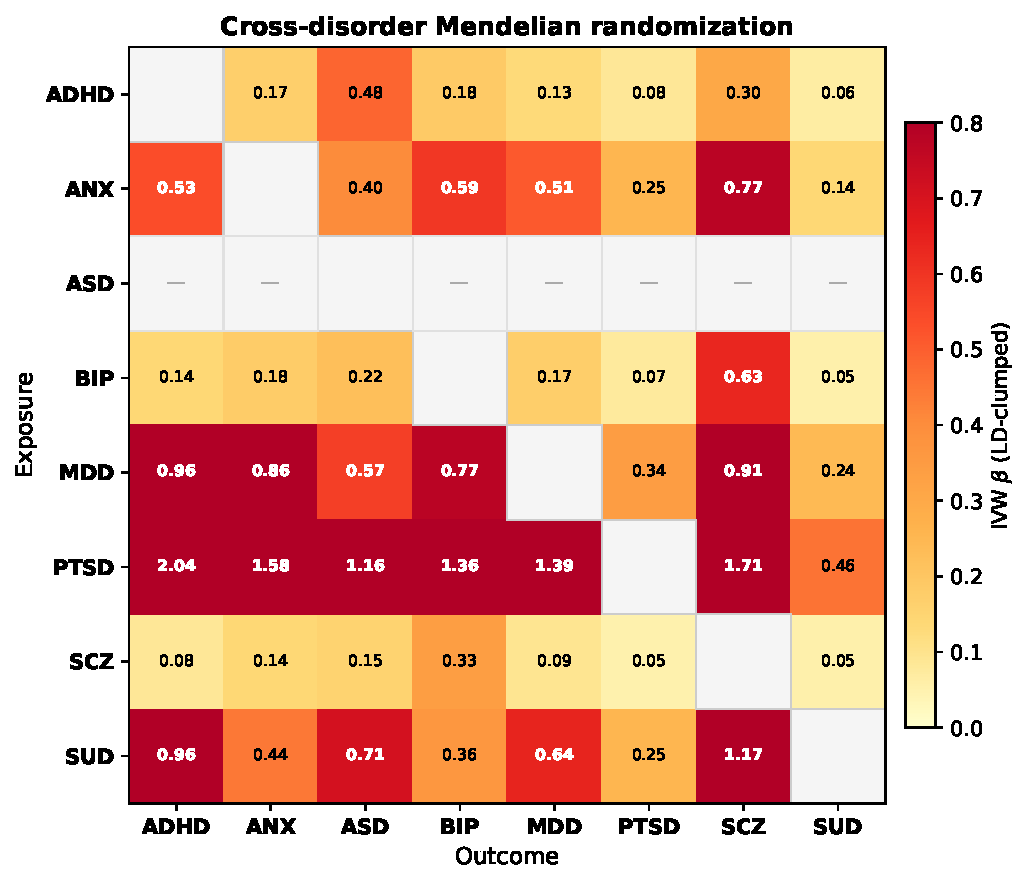
\includegraphics[width=0.72\textwidth]{figures/fig4_mr_heatmap.pdf}
\caption{IVW beta estimates for 49 significant cross-disorder MR pairs. All betas are positive. Dashes (---) indicate the 7 missing ASD-as-exposure pairs (insufficient instruments after LD clumping). Diagonal cells are self-pairs. ASD columns (as outcome) show the weakest effects. PTSD-as-exposure betas are inflated by Z-to-beta conversion (\S\ref{sec:limitations}).}
\label{fig:mr}
\end{figure}

Three patterns are consistent with the curvature results. The MR analysis uses the original 8 psychiatric GWAS (predating the catalog expansion); the expanded graph's new cross-domain entries (sleep, metabolic, autoimmune, thyroid) introduce families without corresponding GWAS in this analysis. Because the network and MR both derive from the same disorder--mechanism catalog, these alignments are expected under a coherent picture rather than independent evidence for it:

\emph{Universal positive pleiotropy parallels negative curvature.} The network's pervasive negative curvature at family--mechanism edges and MR's universal positive genetic overlap both index the same phenomenon: psychiatric mechanisms are shared across disorders. This universal positive pleiotropy is already established by LDSC-based genetic correlation analyses \citep{buliksullivan2015atlas, anttila2018analysis}; our MR results are consistent with those findings and with the catalog's modal failure mode (C4, non-specificity, 12/47 core entries).

\emph{ASD's isolation appears in both.} ASD has 2 independent instruments after clumping and cannot serve as MR exposure. As outcome, ASD shows the weakest MR effects. This parallels the curvature finding: ASD's mechanisms (synaptic pruning $z = +3.21$, MIA/prenatal $z = +3.45$) are the most encapsulated in the network. The Brainstorm Consortium \citep{anttila2018analysis} reported that psychiatric disorders share extensive common-variant risk while neurological disorders do not; ASD sits at the boundary.

\emph{Depression's dominance is edge-specific.} Depression's centrality in MR (largest number of significant pairs as exposure) could reflect its large GWAS sample size (371,184 cases). Edge-level curvature shows where the specificity lies: depression's connections to the convergence hub ($z = -5.46$), metabolic pathways ($z = -3.93$), and circadian mechanisms ($z = -2.62$) are the bottleneck edges whose negative curvature far exceeds degree expectations.

\section{Robustness}
\label{sec:robustness}

The case-study findings rest on the literature-derived catalog, so their credibility depends on whether they survive perturbations to the input.

\paragraph{Catalog perturbation.} We subsampled 85\% of entries (71/84) 100 times, rebuilt the network from each subsample, and recomputed edge-level $z$-scores against 20 degree-preserving permutations per subsample. An edge ``survives'' if $|z| > 1.96$ in that iteration. Depression's bottleneck edges are the most robust structures in the expanded graph: depression--convergence hub survives 100\% of subsamples, depression--metabolic survives 100\%, and depression--circadian survives 76.3\%. The bipolar--metabolic bottleneck survives 81.8\%. Among redundant edges, IL-6/inflammation--Inflammation survives 71.4\% and FKBP5--claim~015 survives 60.6\%.

\paragraph{Leave-one-family-out.} We dropped each of 15 families with $\geq 2$ entries and recomputed edge $z$-scores (50 permutations each). Dropping Depression reduces significant edges from 32 to 3 (9\% survival)---the largest impact of any single family, consistent with depression's role as the convergence bottleneck. Dropping Sleep-Mood leaves only 2/32 (6\%), reflecting its tight coupling to the circadian mechanism. Dropping Anxiety preserves the most edges (6/32, 19\%). The low overall survival rates reflect the expanded graph's denser interconnection: each family contributes to more edges, so dropping any one has ripple effects.

\paragraph{Edge betweenness comparison.} Edge curvature correlates with edge betweenness centrality at $r = -0.674$ ($\rho = -0.633$, both $p < 10^{-4}$). The correlation is weaker than in the original 47-entry graph ($r = -0.79$), because the expanded graph's new domain-specific clusters (autoimmune, thyroid, microbiome) introduce many low-betweenness, high-curvature edges that reduce the linear relationship. Curvature's advantage is clearest for redundant clusters: the autoimmune cluster ($z = +9.40$) has anomalously positive curvature but unremarkable betweenness, because its dense neighborhood overlap produces high curvature while few global shortest paths traverse it.

\section{Related Work}

\paragraph{Discrete curvature on biological networks.} Ollivier-Ricci curvature has been applied to brain structural connectivity \citep{farooq2019network}, cancer gene co-expression \citep{sandhu2015graph}, autism functional connectivity \citep{simhal2020measuring, elumalai2022graph}, and community detection \citep{ni2019community, sia2019ollivier}. Gosztolai and Arnaudon (\citeyear{gosztolai2021unfolding}) developed a dynamical formulation for multiscale analysis. Forman-Ricci curvature \citep{sreejith2016forman} provides a cheaper combinatorial alternative; Samal et al.\ (\citeyear{samal2018comparative}) compared the two discretizations systematically. The dependence of ORC on degree and other centralities is documented: Ni et al.\ (\citeyear{ni2015ricci}) showed that curvature tracks degree, clustering, and betweenness in Internet topology. Park et al.\ (\citeyear{park2025degreecorrected}) proposed a degree-corrected Ricci curvature for community detection. Our contribution is the systematic application of edge-level curvature with null models across multiple biomedical networks---the degree confound itself is known, but the standard practice of reporting node-level curvature without a null persists across the field.

\paragraph{Network psychopathology.} Borsboom (\citeyear{borsboom2017network}) articulated the network theory of mental disorders: disorders arise from symptom--symptom interactions rather than latent common causes. Cramer et al.\ (\citeyear{cramer2010comorbidity}) proposed that comorbidity reflects bridging connections between disorder-specific symptom clusters. Borsboom et al.\ (\citeyear{borsboom2021network}) provide a tutorial on estimation and interpretation. McNally (\citeyear{mcnally2016can}) evaluated whether network reframing can transform psychiatric nosology. Our network operates at the mechanism level (biological substrates) rather than the symptom level (clinical presentation), making curvature a statement about shared biology rather than shared phenomenology.

\paragraph{Cross-disorder genetics.} The Cross-Disorder Group (\citeyear{crossdisorder2013identification, crossdisorder2019genomic}) identified shared risk loci across psychiatric disorders. The Brainstorm Consortium \citep{anttila2018analysis} quantified genetic sharing and found psychiatric disorders cluster while neurological disorders do not. Lee et al.\ (\citeyear{lee2022genetic}) identified latent factors (neurodevelopmental, compulsive, psychotic, internalizing) via genomic SEM. Our MR analysis complements these GWAS meta-analyses by testing directional genetic influence between all disorder pairs rather than static correlations.

\paragraph{Mendelian randomization methodology.} Burgess et al.\ (\citeyear{burgess2013mendelian}) introduced the IVW estimator for two-sample MR. Bowden et al.\ developed MR-Egger (\citeyear{bowden2015mendelian}) and the weighted median estimator (\citeyear{bowden2016consistent}). Hemani et al.\ (\citeyear{hemani2017orienting}) introduced Steiger directionality filtering. Davey Smith and Hemani (\citeyear{daveysmith2014mendelian}) reviewed the broader MR framework including bidirectional and network designs. LD Score regression \citep{buliksullivan2015ld, buliksullivan2015atlas} provides genetic correlation estimators less sensitive to instrument selection; we use published LDSC $r_g$ values in \S\ref{sec:replication} to construct independent weighted graphs for curvature replication.

\section{Limitations}
\label{sec:limitations}

\paragraph{Node curvature reduces to degree.} On an unweighted graph, Ollivier-Ricci curvature for an edge depends entirely on neighborhood overlap. For high-degree nodes, negative curvature is near-tautological. Our permutation test confirms this ($r = -0.71$) on the curated graph. The LDSC graph (\S\ref{sec:replication}) demonstrates the weighted extension, where curvature incorporates transport costs proportional to $|r_g|$, but node-level curvature loses its degree confound only because the graph is nearly complete and degree variance is low ($r = 0.07$, $p = 0.83$).

\paragraph{LDSC graph density.} The LDSC disorder-disorder graph is 65\% dense (36 of 55 possible edges at $p < 0.05$), leaving little room for degree-preserving rewiring. Our weight-permutation null is appropriate for this density regime but tests a different hypothesis (weight--topology association) than the curated graph's degree-preserving null (topology alone). Cross-domain versus within-domain comparisons are significant, but no individual edge reaches significance against the weight-permutation null.

\paragraph{Scope.} This analysis tests the curvature pattern across seven graphs, three disease domains, and five data types. The psychiatric domain is covered by five independent graphs (curated mechanisms, LDSC, shared loci, comorbidity ORs, WHO WMH hazard ratios); autoimmune and cardiometabolic domains have one graph each. Generalizability to additional domains (oncology, neurological) and network types (symptom networks \citep{borsboom2021network}, protein-protein interaction networks) remains untested.

\paragraph{Network construction.} The curated mechanism network reflects literature-derived curation (84 entries: 47 core psychiatric + 37 cross-domain MR), distinct from data-driven clustering. Adding or removing entries changes the topology. Edges are binary; there are no weights for effect size or confidence. The catalog is depression-heavy (15 core entries, plus many cross-domain entries targeting depression), and depression's centrality as a convergence bottleneck may partly reflect attention bias in the psychiatric literature. The catalog-perturbation analysis (\S\ref{sec:robustness}) shows that depression's bottleneck edges survive 100\% of perturbations, making this the most robust finding; domain-specific edges are more fragile.

\paragraph{Verdict-curvature structure.} The Disconfirmed-versus-rest comparison is significant ($p = 0.007$, $d = 0.89$), but the gradient above Disconfirmed is flat. Curvature predicts epistemic failure; it is silent about gradations of success. The 12 Disconfirmed claims may share structural features beyond low curvature (such as targeting the same mechanisms or belonging to depression-dominated families), so the curvature--verdict association may partly reflect catalog composition rather than a general principle.

\paragraph{Verdict prediction ceiling.} The LOOCV classifier achieves AUC $= 0.61$, which is above chance but far from diagnostic. This ceiling reflects the fundamental mismatch between structural features (topology) and the epistemic quality they predict (verdict). Many Disconfirmed claims fail for content-level reasons (weak statistical power, confounding, reverse causation) that graph structure cannot capture.

\paragraph{MR--network non-independence.} The MR analysis tests genetic relationships between disorder pairs that also structure the network. Both derive from the same disorder--mechanism catalog, so their alignment constitutes a consistency check rather than independent validation. The universal positive pleiotropy we observe is already established by LDSC genetic correlation analyses \citep{buliksullivan2015atlas, anttila2018analysis}; our MR adds directional estimates but does not test the geometry per se.

\paragraph{ASD missing from MR.} The 2019 ASD GWAS \citep{grove2019identification} yields only $\sim$5 genome-wide significant loci, which reduce to $<3$ independent instruments after 10\,Mb distance-based clumping. This removes 7/56 pairs (all ASD-as-exposure). A larger ASD GWAS would close this gap.

\paragraph{PTSD scale.} The PTSD GWAS reports $Z$-scores rather than log-odds ratios. Our $Z \to \beta$ conversion ($\beta = Z / \sqrt{2 \cdot \text{EAF} \cdot (1 - \text{EAF}) \cdot N}$) inflates PTSD-as-exposure betas (1.0--2.0) relative to OR-scale GWAS. Directional significance is valid; magnitude comparisons across disorders are not.

\paragraph{LD pruning and sample overlap.} We used 10\,Mb distance windows rather than reference-panel LD clumping---conservative (removes more instruments than necessary) but may miss long-range LD. Several GWAS share UK Biobank participants; overlap biases MR toward the null \citep{hemani2018mrbase}, so positive findings are conservative, but estimates may be attenuated.

\paragraph{Edge-level multiple comparisons.} We test 103 edges (those with sufficient null samples) at $\alpha = 0.05$, yielding an expected false-positive count of $\sim$5.2 under the global null. Of 32 reported edges, those near $|z| \approx 2.0$ may be false discoveries. The strongest edges (depression--convergence $z = -5.46$, autoimmune cluster $z = +9.40$) survive Benjamini-Hochberg correction \citep{benjamini1995controlling}; marginal edges should be treated as hypothesis-generating.

\section{Conclusion}

Edge-level Ollivier-Ricci curvature, paired with degree-preserving or weight-permutation null models, decomposes bridge and redundancy structure in disease networks that node-level curvature cannot resolve. Node-level ORC is a degree artifact ($r = -0.71$); the standard practice of reporting it without a null model, which persists across biomedical applications, produces misleading bottleneck narratives.

The method replicates across six data-driven graphs spanning four data types and three disease domains, with a concordant pattern in the curated mechanism network (seven graphs total across five data types). Within-cluster edges have higher curvature than cross-cluster edges in all seven (4/6 data-driven significant, $d = 0.46$--$1.55$). In every graph, the lowest-curvature node is a recognized bridge entity connecting established diagnostic groupings through weak inter-cluster connections.

Applied to a 130-node psychiatric mechanism network, the method identifies four bottleneck edges, all involving depression or bipolar disorder bridging cross-domain mechanisms. Depression's bottleneck edges survive 100\% of catalog perturbations. Disconfirmed claims occupy significantly lower-curvature positions than higher-verdict claims ($p = 0.007$, $d = 0.89$), and among five edge-level methods, only ORC achieves this discrimination ($d = 0.73$, $p = 0.011$). The AUC of 0.61 for cross-validated verdict prediction honestly reflects the ceiling on structural prediction of epistemic quality.

Curvature's advantage over simpler alternatives is its joint sensitivity to neighborhood overlap and divergence, which makes it uniquely suited to detect bridge entities connecting established diagnostic groupings through weak inter-cluster connections. The extension to weighted graphs makes curvature sensitive to information beyond binary topology, a direction that unweighted-only alternatives such as Forman-Ricci curvature \citep{sreejith2016forman} cannot follow.

\paragraph{Data and code availability.} All GWAS summary statistics are publicly available from the Psychiatric Genomics Consortium (\url{https://pgc.unc.edu}). The mechanism catalog, analysis code, precomputed curvatures, permutation distributions, and MR results are available at \url{https://github.com/elliottower/psychiatric-comorbidity-curvature}, with a DOI-versioned snapshot archived at \url{https://doi.org/10.5281/zenodo.21251608}.

\bibliographystyle{unsrtnat}
\bibliography{references}

\appendix

\section{Full MR Results}
\label{app:mr}

Table~\ref{tab:mr_full} reports IVW, MR-Egger, and weighted median estimates for all 49 completed cross-disorder MR pairs. Seven ASD-as-exposure pairs are omitted (insufficient instruments). PTSD-as-exposure betas are inflated by Z-to-beta conversion and should not be compared in magnitude to OR-scale GWAS. Egger intercept $p$-values test for directional pleiotropy; values $< 0.05$ suggest the IVW estimate may be biased. $I^2$ values are available only for pairs with $\geq 25$ instruments.

\begin{table}[h]
\centering
\caption{Full cross-disorder MR results (49 pairs). $k$: number of independent instruments after LD clumping. $^{\dagger}$Egger intercept $p < 0.05$, indicating possible directional pleiotropy; IVW estimate should be interpreted cautiously. PTSD-as-exposure betas are inflated by Z-to-beta conversion (\S\ref{sec:limitations}).}
\label{tab:mr_full}
\footnotesize
\begin{tabular}{llccccccc}
\toprule
Pair & $k$ & IVW $\beta$ & 95\% CI & Egger $\beta$ & Egger int.\ $p$ & WM $\beta$ & $I^2$\% \\
\midrule
ADHD $\to$ ANX & 25 & 0.167 & [0.135, 0.199] & -- & 0.303 & 0.183 & -- \\
ADHD $\to$ ASD & 25 & 0.482 & [0.391, 0.573] & -- & 0.080 & 0.469 & -- \\
ADHD $\to$ BIP & 24 & 0.182 & [0.131, 0.232] & -- & 0.732 & 0.128 & -- \\
ADHD $\to$ MDD & 22 & 0.130 & [0.110, 0.150] & -- & 0.164 & 0.119 & -- \\
ADHD $\to$ PTSD & 24 & 0.084 & [0.073, 0.096] & -- & 0.574 & 0.079 & -- \\
ADHD $\to$ SCZ & 25 & 0.303 & [0.246, 0.359] & -- & 0.174 & 0.259 & -- \\
ADHD $\to$ SUD & 8 & 0.064 & [0.038, 0.089] & -- & 0.597 & 0.071 & -- \\
\midrule
ANX $\to$ ADHD & 47 & 0.535 & [0.446, 0.623] & -- & 0.234 & 0.397 & -- \\
ANX $\to$ ASD & 49 & 0.402 & [0.273, 0.530] & -- & 0.682 & 0.402 & -- \\
ANX $\to$ BIP & 46 & 0.588 & [0.515, 0.660] & -- & 0.637 & 0.531 & -- \\
ANX $\to$ MDD & 43 & 0.509 & [0.480, 0.537] & -- & 0.329 & 0.517 & -- \\
ANX $\to$ PTSD & 46 & 0.251 & [0.234, 0.268] & -- & 0.457 & 0.245 & -- \\
ANX $\to$ SCZ & 48 & 0.773 & [0.692, 0.855] & -- & 0.513 & 0.641 & -- \\
ANX $\to$ SUD & 14 & 0.135 & [0.096, 0.175] & -- & 0.738 & 0.145 & -- \\
\midrule
BIP $\to$ ADHD & 58 & 0.136 & [0.085, 0.187] & -- & 0.707 & 0.126 & -- \\
BIP $\to$ ANX & 55 & 0.176 & [0.148, 0.203] & -- & 0.886 & 0.183 & -- \\
BIP $\to$ ASD & 58 & 0.219 & [0.145, 0.294] & -- & 0.029 & 0.208 & -- \\
BIP $\to$ MDD & 47 & 0.169 & [0.152, 0.186] & -- & 0.084 & 0.167 & -- \\
BIP $\to$ PTSD & 53 & 0.072 & [0.062, 0.082] & -- & 0.955 & 0.064 & -- \\
BIP $\to$ SCZ & 60 & 0.634 & [0.588, 0.680] & -- & 0.532 & 0.613 & -- \\
BIP $\to$ SUD & 14 & 0.050 & [0.026, 0.074] & -- & 0.343 & 0.043 & -- \\
\midrule
MDD $\to$ ADHD & 124 & 0.959 & [0.875, 1.043] & 0.960 & 0.928 & 0.971 & 58 \\
MDD $\to$ ANX & 128 & 0.862 & [0.819, 0.905] & 0.857 & 0.419 & 0.874 & 47 \\
MDD $\to$ ASD & 126 & 0.572 & [0.448, 0.695] & 0.587 & 0.312 & 0.472 & 34 \\
MDD $\to$ BIP$^{\dagger}$ & 126 & 0.774 & [0.708, 0.841] & 0.743 & \textbf{0.008} & 0.803 & 69 \\
MDD $\to$ PTSD & 125 & 0.339 & [0.323, 0.355] & 0.337 & 0.467 & 0.334 & 46 \\
MDD $\to$ SCZ & 128 & 0.909 & [0.833, 0.985] & 0.897 & 0.520 & 0.825 & 85 \\
MDD $\to$ SUD & 59 & 0.240 & [0.210, 0.269] & 0.243 & 0.568 & 0.252 & 68 \\
\midrule
PTSD $\to$ ADHD & 53 & 2.036 & [1.816, 2.256] & -- & 0.950 & 2.223 & -- \\
PTSD $\to$ ANX & 51 & 1.579 & [1.462, 1.696] & -- & 0.710 & 1.624 & -- \\
PTSD $\to$ ASD & 53 & 1.158 & [0.837, 1.480] & -- & 0.367 & 1.111 & -- \\
PTSD $\to$ BIP & 51 & 1.359 & [1.181, 1.536] & -- & 0.582 & 1.623 & -- \\
PTSD $\to$ MDD & 44 & 1.394 & [1.320, 1.468] & -- & 0.447 & 1.318 & -- \\
PTSD $\to$ SCZ & 54 & 1.706 & [1.506, 1.905] & -- & 0.564 & 1.810 & -- \\
PTSD $\to$ SUD & 25 & 0.455 & [0.383, 0.527] & -- & 0.395 & 0.498 & -- \\
\midrule
SCZ $\to$ ADHD & 105 & 0.083 & [0.054, 0.113] & -- & 0.858 & 0.083 & -- \\
SCZ $\to$ ANX & 103 & 0.137 & [0.122, 0.153] & -- & 0.674 & 0.128 & -- \\
SCZ $\to$ ASD & 106 & 0.153 & [0.109, 0.196] & -- & 0.981 & 0.137 & -- \\
SCZ $\to$ BIP & 103 & 0.334 & [0.310, 0.359] & -- & 0.115 & 0.326 & -- \\
SCZ $\to$ MDD & 98 & 0.091 & [0.082, 0.100] & -- & 0.754 & 0.097 & -- \\
SCZ $\to$ PTSD & 102 & 0.050 & [0.044, 0.055] & -- & 0.719 & 0.046 & -- \\
SCZ $\to$ SUD & 55 & 0.051 & [0.041, 0.061] & -- & 0.683 & 0.042 & -- \\
\midrule
SUD $\to$ ADHD & 15 & 0.963 & [0.629, 1.296] & -- & 0.844 & 1.338 & -- \\
SUD $\to$ ANX & 15 & 0.443 & [0.275, 0.610] & -- & 0.062 & 0.498 & -- \\
SUD $\to$ ASD & 15 & 0.709 & [0.219, 1.198] & -- & 0.645 & 0.896 & -- \\
SUD $\to$ BIP & 14 & 0.362 & [0.089, 0.634] & -- & 0.051 & 0.412 & -- \\
SUD $\to$ MDD & 13 & 0.638 & [0.532, 0.745] & -- & 0.731 & 0.960 & -- \\
SUD $\to$ PTSD & 15 & 0.250 & [0.188, 0.313] & -- & 0.643 & 0.209 & -- \\
SUD $\to$ SCZ & 15 & 1.166 & [0.862, 1.469] & -- & 0.756 & 0.378 & -- \\
\bottomrule
\end{tabular}
\end{table}

\section{Significant Edge-Level Curvature $z$-Scores}
\label{app:edges}

Table~\ref{tab:edge_full} lists the 32 edges with $|z| > 1.96$ against the degree-preserving null (200 permutations) in the expanded 84-entry graph. All four bottleneck edges involve depression or bipolar disorder bridging cross-domain mechanisms. The 28 redundant edges include domain-specific clusters (autoimmune, thyroid, microbiome) and encapsulated claims.

\begin{table}[h]
\centering
\caption{Significant edge-level curvature $z$-scores (32 of 103 tested edges). Sorted by $z$-score.}
\label{tab:edge_full}
\small
\begin{tabular}{lccc}
\toprule
Edge & $\kappa_{\text{obs}}$ & $z$ \\
\midrule
\multicolumn{3}{l}{\emph{Bottleneck edges ($z < -1.96$)}} \\
Depression -- convergence hub & $-0.867$ & $\mathbf{-5.46}$ \\
Depression -- metabolic & $-0.780$ & $\mathbf{-3.93}$ \\
Bipolar -- metabolic & $-0.693$ & $-3.33$ \\
Depression -- circadian & $-0.675$ & $-2.62$ \\
\midrule
\multicolumn{3}{l}{\emph{Top redundant edges ($z > +1.96$; 28 total)}} \\
Autoimmune cluster & $+0.583$ & $\mathbf{+9.40}$ \\
FKBP5 -- claim 004 & $+0.167$ & $+5.09$ \\
ASD -- claim 037-inst & $+0.167$ & $+4.15$ \\
HPA axis -- claim 004 & $+0.104$ & $+4.09$ \\
Thyroid-Metabolic -- thyroid & $+0.100$ & $+3.60$ \\
Microbiome -- gut-brain & $+0.267$ & $+3.43$ \\
Anxiety -- claim 023 & $+0.000$ & $+3.39$ \\
Autoimmune -- claim 076 & $+0.250$ & $+3.38$ \\
Sleep-Mood -- circadian & $+0.100$ & $+3.26$ \\
Schizophrenia -- claim 029 & $-0.015$ & $+3.14$ \\
\bottomrule
\end{tabular}
\end{table}

\section{Mechanism Catalog}
\label{app:catalog}

Table~\ref{tab:catalog} lists all 47 entries in the literature-derived catalog from which the mechanism network is constructed. Verdict tiers range from Disconfirmed (lowest) to Validated (highest). Shared mechanism nodes link claims across disorder families; entries with no shared nodes connect only to their disorder family.

\begin{table}[h]
\centering
\caption{Full mechanism catalog (47 entries). Verdict tiers: D = Disconfirmed, U = Underdetermined, I = Inconclusive, CS = Causally Suggestive, MS = Mechanistically Supported, V = Validated.}
\label{tab:catalog}
\footnotesize
\begin{tabular}{llll}
\toprule
ID & Family & Verdict & Shared mechanisms \\
\midrule
001 & Depression & D & -- \\
003 & Depression & D & Serotonin \\
004 & Depression & D & HPA axis, FKBP5 \\
006a & Depression & CS & IL-6 \\
006b & Depression & D & IL-6 \\
008 & Depression & D & -- \\
008b & Depression & MS & -- \\
010 & Depression & I & -- \\
011 & Depression & CS & NMDA/Glu, IL-6 \\
012 & Depression & U & NMDA/Glu \\
012a & Depression & MS & NMDA/Glu \\
013 & Depression & U & Mitochondrial \\
014 & Depression & CS & Circadian \\
015 & Depression & CS & FKBP5, HPA axis \\
016 & Depression & CS & -- \\
\midrule
017 & PTSD & CS & FKBP5, HPA axis \\
018 & PTSD & MS & Fear circuit \\
019 & PTSD & CS & Noradrenergic \\
020 & PTSD & U & HPA axis \\
\midrule
021a & Anxiety & V & -- \\
021b & Anxiety & D & -- \\
022 & Anxiety & MS & Fear circuit \\
023 & Anxiety & D & Serotonin \\
024 & Anxiety & CS & Noradrenergic \\
\midrule
025 & Schizophrenia & MS & Dopamine \\
025-orig & Schizophrenia & D & Dopamine \\
026 & Schizophrenia & CS & NMDA/Glu \\
027 & Schizophrenia & MS & Syn.\ pruning \\
028 & Schizophrenia & CS & MIA/prenatal \\
029 & Schizophrenia & CS & MIA/prenatal, IL-6 \\
\midrule
030 & Bipolar & CS & Mitochondrial \\
031a & Bipolar & CS & Circadian \\
031b & Bipolar & D & Circadian \\
032 & Bipolar & CS & -- \\
033 & Bipolar & I & -- \\
\midrule
034 & OCD & MS & CSTC circuit \\
035 & OCD & D & Serotonin \\
036 & OCD & U & NMDA/Glu \\
\midrule
037 & ASD & CS & NMDA/Glu \\
037-inst & ASD & MS & NMDA/Glu, Syn.\ pruning \\
038 & ASD & CS & MIA/prenatal, IL-6 \\
039 & ASD & MS & Syn.\ pruning \\
\midrule
040 & Addiction & MS & Dopamine \\
041 & Addiction & CS & HPA axis \\
042 & Addiction & CS & Dopamine \\
\midrule
043 & ADHD & CS & Noradrenergic, Dopamine \\
044 & ADHD & CS & -- \\
\bottomrule
\end{tabular}
\end{table}

\section{Robustness Details}
\label{app:robustness}

Table~\ref{tab:perturbation} reports catalog-perturbation survival rates for the expanded 84-entry graph (100 subsamples of 71/84 entries, 20 null permutations per subsample).

\begin{table}[h]
\centering
\caption{Catalog perturbation survival rates (100 subsamples of 71/84 entries). Survival = fraction of iterations where the edge reaches $|z| > 1.96$. Only edges with $> 50\%$ survival shown.}
\label{tab:perturbation}
\small
\begin{tabular}{lcc}
\toprule
Edge & Survival & Present \\
\midrule
\multicolumn{3}{l}{\emph{Bottleneck edges}} \\
Depression--convergence hub & 100.0\% & 99 \\
Depression--metabolic & 100.0\% & 96 \\
Bipolar--metabolic & 81.8\% & 22 \\
Depression--circadian & 76.3\% & 97 \\
\midrule
\multicolumn{3}{l}{\emph{Redundant edges}} \\
Claim 011--Depression & 78.1\% & 32 \\
IL-6--Inflammation & 71.4\% & 14 \\
Claim 015--Depression & 60.6\% & 33 \\
Depression--IL-6/inflammation & 53.0\% & 100 \\
\bottomrule
\end{tabular}
\end{table}

\section{Expanded Catalog: Cross-Domain Entries}
\label{app:expanded}

Table~\ref{tab:expanded} lists the 37 cross-domain MR entries added to the core 47-entry catalog. These entries span sleep--mood, metabolic, personality, substance use, inflammation, microbiome, thyroid, autoimmune, and neuroimaging domains.

\begin{table}[h]
\centering
\caption{Cross-domain MR catalog entries (37 entries). Verdict abbreviations as in Table~\ref{tab:catalog}.}
\label{tab:expanded}
\footnotesize
\begin{tabular}{llll}
\toprule
ID & Family & Verdict & Shared mechanisms \\
\midrule
045--048 & Sleep-Mood & CS/U & Circadian \\
049 & Eating & MS & Metabolic \\
050 & Eating-Mood & CS & Metabolic \\
051 & Personality & MS & Depression convergence \\
052--053 & Personality-Social, Social & CS & Depression convergence \\
054 & Substance-Neurodev & MS & Dopamine \\
055 & Substance-Mood & CS & Depression convergence \\
056 & Substance & U & -- \\
057 & Neurodev-Mood & CS & Depression convergence \\
058 & Stress-Mood & CS & FKBP5 \\
059--061 & Inflammation & CS/D & IL-6/inflammation \\
062--063 & Microbiome & U & Microbiome-gut-brain \\
064 & Mediator & MS & IL-6/inflammation \\
065 & Microbiome-Neuro & CS & Microbiome-gut-brain \\
066--068 & Thyroid-Metabolic & CS/U & Metabolic \\
069--072 & Thyroid-Metabolic & CS/D & Thyroid \\
073 & Thyroid-Metabolic & CS & Metabolic \\
074--078 & Autoimmune & CS/MS/U & Autoimmune \\
079--081 & Neuroimaging-endo & CS & Neuroimaging \\
\bottomrule
\end{tabular}
\end{table}

\end{document}
